\section{Рабочий проект}

\subsection{Описание классов системы}

\subsubsection{Описание программных классов серверной части}

\begin{itemize}
    \item <<UserBase>> является фундаментальным классом для хранения пользовательских данных. Помимо основных свойств, таких как <<Phone>>, <<Email>>, <<FirstName>>, <<LastName>>, предлагает основу для дальнейшего расширения и интеграции с другими подсистемами приложения;
    \item <<UserRegistrationData>> расширяет <<UserBase>>, вводя специфические свойства, необходимые для процесса регистрации, включая <<Password>>. Это обеспечивает дополнительный уровень безопасности и индивидуализации данных пользователя;
    \item <<UserLoginData>> применяется для авторизации пользователей в системе. Содержит только самую необходимую информацию для входа, а именно: <<Email>> и <<Password>>;
    \item <<UserLoginResponseData>> и <<UserView>> наследуются от <<UserBase>> и дополняют его уникальным идентификатором <<Id>>. <<UserLoginResponseData>> также включает в себя <<AccessToken>>, что обеспечивает надежную аутентификацию и безопасность данных;
    \item <<User>> представляет собой полную структуру класса пользователя, включая элементы безопасности (<<Hash>> и <<Salt>>) и уникальный идентификатор <<Id>>. Этот класс является центральным в системе управления пользователями и их данными.
\end{itemize}
 
\renewcommand{\arraystretch}{0.8} % уменьшение расстояний до сетки таблицы

% Таблица для HashSalt
\begin{xltabular}{\textwidth}{|l|l|p{1.7cm}|X|}
    \caption{Свойства класса <<HashSalt>>}\label{hashsalt:table} \\ \hline
    Свойство & Тип & \makecell{Обяза-\\тельное} & Описание \\ \hline
    1 & 2 & 3 & 4 \\ \hline
    \finishhead
    Hash & String & true & Хэш \\ \hline
    Salt & String & true & Соль для хэша \\
\end{xltabular}

% Таблица для UserBase
\begin{xltabular}{\textwidth}{|l|l|p{1.7cm}|X|}
    \caption{Свойства класса <<UserBase>>}\label{userbase:table} \\ \hline
    Свойство & Тип & \makecell{Обяза-\\тельное} & Описание \\ \hline
    1 & 2 & 3 & 4 \\ \hline
    \endfirsthead
    1 & 2 & 3 & 4 \\ \hline
    \finishhead
    Phone & String & false & Телефонный номер пользователя \\ \hline
    Email & String & false & Электронная почта пользователя \\ \hline
    FirstName & String & false & Имя пользователя \\ \hline
    LastName & String & false & Фамилия пользователя \\ \hline
    ImageUrl & String & false & URL изображения пользователя \\ \hline
    Telegram & String & false & Telegram пользователя \\ \hline
    Website & String & false & Веб-сайт пользователя \\
\end{xltabular}

% Таблица для UserRegistrationData
\begin{xltabular}{\textwidth}{|l|l|p{1.7cm}|X|}
    \caption{Свойства класса <<UserRegistrationData>>}\label{userregdata:table} \\ \hline
    Свойство & Тип & \makecell{Обяза-\\тельное} & Описание \\ \hline
    1 & 2 & 3 & 4 \\ \hline
    Password & String & true & Пароль пользователя \\ \hline
\end{xltabular}

% Таблица для UserLoginData
\begin{xltabular}{\textwidth}{|l|l|p{1.7cm}|X|}
    \caption{Свойства класса <<UserLoginData>>}\label{userlogindata:table} \\ \hline
    Свойство & Тип & \makecell{Обяза-\\тельное} & Описание \\ \hline
    1 & 2 & 3 & 4 \\ \hline
    Email & String & true & Электронная почта пользователя для входа \\ \hline
    Password & String & true & Пароль пользователя для входа \\ \hline
\end{xltabular}



% Таблица для UserLoginResponseData
\begin{xltabular}{\textwidth}{|l|l|p{1.7cm}|X|}
    \caption{Свойства класса <<UserLoginResponseData>>}\label{userloginrespdata:table} \\ \hline
    Свойство & Тип & \makecell{Обяза-\\тельное} & Описание \\ \hline
    1 & 2 & 3 & 4 \\ \hline
    Id & Long & true & Уникальный идентификатор пользователя \\ \hline
    AccessToken & String & true & Токен доступа пользователя \\ \hline
\end{xltabular}

% Таблица для UserView
\begin{xltabular}{\textwidth}{|l|l|p{1.7cm}|X|}
    \caption{Свойства класса <<UserView>>}\label{userview:table} \\ \hline
    Свойство & Тип & \makecell{Обяза-\\тельное} & Описание \\ \hline
    1 & 2 & 3 & 4 \\ \hline
    Id & Long & true & Уникальный идентификатор пользователя \\ \hline
\end{xltabular}

% Таблица для User
\begin{xltabular}{\textwidth}{|l|l|p{1.7cm}|X|}
    \caption{Свойства класса <<User>>}\label{user:table} \\ \hline
    Свойство & Тип & \makecell{Обяза-\\тельное} & Описание \\ \hline
    1 & 2 & 3 & 4 \\ \hline
    \endfirsthead
    1 & 2 & 3 & 4 \\ \hline
    \finishhead
    Id & Long & true & Уникальный идентификатор пользователя \\ \hline
    Hash & String & true & Хэш пользователя \\ \hline
    Salt & String & true & Соль для хэша пароля пользователя \\
\end{xltabular}

\renewcommand{\arraystretch}{1.0} % восстановление сетки

Большой набор классов для описания пользователя в серверной части приложение таких как <<UserBase>>, <<UserRegistrationData>>, <<UserLoginData>>, <<UserLoginResponseData>> и <<User>>, подчеркивает разнообразие и сложность структур данных в современных системах. Подход к проектированию \cite{grinchenko} и реализации этих классов основывается на объектно-ориентированных принципах и практиках \cite{kumskova}.

В частности, класс <<User>> является центральным в системе управления пользователями и их данными, что подчеркивает важность его реализации и интеграции с другими классами.

\renewcommand{\arraystretch}{0.8} % уменьшение расстояний до сетки таблицы

% Таблица для Product
\begin{xltabular}{\textwidth}{|l|l|p{1.7cm}|X|}
    \caption{Свойства класса <<Product>>}\label{product:table} \\ \hline
    Свойство & Тип & \makecell{Обяза-\\тельное} & Описание \\ \hline
    1 & 2 & 3 & 4 \\ \hline
    \endfirsthead
    \hline 1 & 2 & 3 & 4 \\ \hline
    \finishhead
    ImageUrl & String & false & URL изображения продукта \\ \hline
    ProductGroupId & Long & true & Идентификатор группы продуктов \\ \hline
    Price & Float & true & Цена продукта \\ \hline
    Weight & Integer & true & Вес продукта \\ \hline
    CreatedByUserId & Long & true & Идентификатор пользователя, создавшего продукт \\
\end{xltabular}

% Таблица для ProductView
\begin{xltabular}{\textwidth}{|l|l|p{1.7cm}|X|}
    \caption{Свойства класса <<ProductView>>}\label{productview:table} \\ \hline
    Свойство & Тип & \makecell{Обяза-\\тельное} & Описание \\ \hline
    1 & 2 & 3 & 4 \\ \hline
    CreatedByUser & UserView & true & Пользователь, создавший продукт \\ \hline
\end{xltabular}

\renewcommand{\arraystretch}{1}

\begin{itemize}
    \item <<Product>>, наследующийся от <<Short>>, описывает основные свойства продукта, такие как <<ImageUrl>>, <<ProductGroupId>>, <<Price>>, <<Weight>>, и <<CreatedByUserId>>, указывающий на пользователя, создавшего продукт;
    \item <<ProductView>> расширяет <<Product>>, добавляя <<CreatedByUser>>, который является экземпляром <<UserView>>. Это позволяет получать не только идентификационную информацию о создателе продукта, но и более детальные данные пользователя.
\end{itemize}



\renewcommand{\arraystretch}{0.8} % уменьшение расстояний до сетки таблицы

% Таблица для IUserRepository
\begin{xltabular}{\textwidth}{|l|l|p{1.7cm}|X|}
    \caption{Свойства класса <<IUserRepository>>}\label{iuserrepository:table} \\ \hline
    Свойство & Тип & \makecell{Обяза-\\тельное} & Описание \\ \hline
    1 & 2 & 3 & 4 \\ \hline
    \endfirsthead
    1 & 2 & 3 & 4 \\ \hline
    \finishhead
    GetById & User & true & Получить пользователя по идентификатору \\ \hline
    GetByEmail & User & true & Получить пользователя по электронной почте \\ \hline
    GetAllUserViews & List<UserView> & true & Получить список пользователей \\ \hline
    Create & User & true & Создать пользователя \\
\end{xltabular}

\renewcommand{\arraystretch}{1}

Класс <<IUserRepository>> описывает основные методы для работы с пользователями, включая получение пользователя по идентификатору, получение пользователя по электронной почте, получение списка пользователей и создание пользователя.

В системе предусмотрен внутренний механизм связи между классами и их свойствами, поэтому введение дополнительных идентификаторов при реализации связей между классами не предполагается.

Экземпляры классов реализуются в информационных блоках посредством элементов, свойства класса – посредством свойств и методов элемента.

\subsubsection{Описание программных классов клиентской части}

\begin{itemize}
    \item <<Short>> - основной класс, используемый для предоставления общей структуры данных. Свойства <<id>>, <<name>> и <<description>> являются фундаментальными для большинства классов;
    \item <<User>> - расширяет <<Short>>, интегрируя контактные данные и личную информацию пользователя. Используется для управления учетными записями пользователей, включая процессы регистрации и авторизации;
    \item <<ProductGroup>> - расширяет <<Short>>, добавляя конкретные детали для организации продуктов в группы. Используется для классификации и управления ассортиментом продуктов;
    \item <<Product>> - расширяет <<Short>>, предоставляя подробную информацию о продуктах. Включает данные о создателе продукта и используется для представления конкретных товаров в системе;
    \item <<City>> - описывает города, со свойствами <<id>> и <<name>>. Используется для управления информацией о местоположениях, связанных с пользователями и продуктами;
    \item <<ProductFilter>> - используется для фильтрации продуктов по городу, группе продуктов, дате публикации и дате окончания срока действия.
\end{itemize}

\renewcommand{\arraystretch}{0.8} % уменьшение расстояний до сетки таблицы

% Таблица для Short
\begin{xltabular}{\textwidth}{|l|l|p{1.7cm}|X|}
    \caption{Свойства класса <<Short>>\label{int1:table}}\\ \hline
    Свойство & Тип & \makecell{Обяза-\\тельное} & Описание \\ \hline
    1 & 2 & 3 & 4 \\ \hline
    \endfirsthead
    1 & 2 & 3 & 4 \\ \hline
    \finishhead
    id & number & true & Уникальный идентификатор \\ \hline
    name & string & true & Название \\ \hline
    description & string & true & Описание \\
\end{xltabular}

% Таблица для User
\begin{xltabular}{\textwidth}{|l|l|p{1.7cm}|X|}
    \caption{Свойства класса <<User>>\label{int2:table}}\\ \hline
    Свойство & Тип & \makecell{Обяза-\\тельное} & Описание \\ \hline
    1 & 2 & 3 & 4 \\ \hline
    \endfirsthead
    \hline 1 & 2 & 3 & 4 \\ \hline
    \finishhead
    phone & string & true & Телефонный номер \\ \hline
    email & string & true & Электронная почта \\ \hline
    firstName & string & true & Имя \\ \hline
    lastName & string & true & Фамилия \\ \hline
    photoUrl & string & true & URL изображения \\ \hline
    telegram & string & true & Telegram \\ \hline
    website & string & true & Веб-сайт \\ \hline
    address & string & true & Адрес \\ \hline
    userRoleId & number & true & Идентификатор роли \\ \hline
    password & string & false & Пароль пользователя (передается при авторизации и регистрации) \\ \hline
    accessToken & string & false & Токен доступа (принимается при авторизации и регистрации) \\
\end{xltabular}

% Таблица для Product
\begin{xltabular}{\textwidth}{|l|l|p{1.7cm}|X|}
    \caption{Свойства класса <<Product>>\label{int3:table}}\\ \hline
    Свойство & Тип & \makecell{Обяза-\\тельное} & Описание \\ \hline
    1 & 2 & 3 & 4 \\ \hline
    \endfirsthead
    \hline 1 & 2 & 3 & 4 \\ \hline
    \finishhead
    imageUrl & string & true & URL изображения продукта \\ \hline
    productGroupId & number & true & Идентификатор группы продуктов \\ \hline
    price & number & true & Цена продукта \\ \hline
    weight & number & true & Вес продукта \\ \hline
    createdByUserId & number & true & Идентификатор пользователя, создавшего продукт \\ \hline
    publishedAt & Date & true & Дата публикации \\ \hline
    expiredAt & Date & true & Дата окончания срока действия \\
\end{xltabular}

% Таблица для ProductGroup
\begin{xltabular}{\textwidth}{|l|l|p{1.7cm}|X|}
    \caption{Свойства класса <<ProductGroup>>\label{int4:table}}\\ \hline
    Свойство & Тип & \makecell{Обяза-\\тельное} & Описание \\ \hline
    1 & 2 & 3 & 4 \\ \hline
    \endfirsthead
    1 & 2 & 3 & 4 \\ \hline
    \finishhead
    type & string & true & Тип группы продуктов \\ \hline
    childrenProductGroupIds & number[] & true & Идентификаторы дочерних групп продуктов (может быть пустым массивом) \\ \hline
    parentProductGroupId & number & false & Идентификатор родительской группы продуктов \\
\end{xltabular}

% Таблица для ProductFilter
\begin{xltabular}{\textwidth}{|l|l|p{1.7cm}|X|}
    \caption{Свойства класса <<ProductFilter>>\label{int5:table}}\\ \hline
    Свойство & Тип & \makecell{Обяза-\\тельное} & Описание \\ \hline
    1 & 2 & 3 & 4 \\ \hline
    \endfirsthead
    1 & 2 & 3 & 4 \\ \hline
    \finishhead
    cityId & number & false & Идентификатор города \\ \hline
    productGroupId & number & false & Идентификатор группы продуктов \\ \hline
    publishedAtFrom & Date & false & Дата публикации \\ \hline
    expiredAtTo & Date & false & Дата окончания срока действия \\
\end{xltabular}

% Таблица для City
\begin{xltabular}{\textwidth}{|l|l|p{1.7cm}|X|}
    \caption{Свойства класса <<City>>\label{int6:table}}\\ \hline
    Свойство & Тип & \makecell{Обяза-\\тельное} & Описание \\ \hline
    1 & 2 & 3 & 4 \\ \hline
    \endfirsthead
    1 & 2 & 3 & 4 \\ \hline
    \finishhead
    id & number & true & Уникальный идентификатор \\ \hline
    name & string & true & Название города \\
\end{xltabular}

% Таблица для UserService
\begin{xltabular}{\textwidth}{|l|l|p{1.7cm}|X|}
    \caption{Свойства класса <<UserService>>\label{int6:table}}\\ \hline
    Свойство & Тип & \makecell{Обяза-\\тельное} & Описание \\ \hline
    1 & 2 & 3 & 4 \\ \hline
    \endfirsthead
    1 & 2 & 3 & 4 \\ \hline
    \finishhead
    getById & User & true & Получить пользователя по идентификатору \\ \hline
    login & User & true & Получить пользователя по электронной почте \\ \hline
    create & User & true & Получить список пользователей \\ \hline
    update & User & true & Создать пользователя \\ \hline
\end{xltabular}

% Таблица для ProductGroupService
\begin{xltabular}{\textwidth}{|l|l|p{1.7cm}|X|}
    \caption{Свойства класса <<ProductGroupService>>\label{int7:table}}\\ \hline
    Метод & Тип & \makecell{Обяза-\\тельное} & Описание \\ \hline
    1 & 2 & 3 & 4 \\ \hline
    \endfirsthead
    1 & 2 & 3 & 4 \\ \hline
    \finishhead
    getAll & ProductGroup[] & true & Получить все группы продуктов \\ \hline
    updateAll & ProductGroup[] & true & Обновить все группы продуктов \\
\end{xltabular}

% Таблица для ProductService
\begin{xltabular}{\textwidth}{|l|l|p{1.7cm}|X|}
    \caption{Свойства класса <<ProductService>>\label{int8:table}}\\ \hline
    Метод & Тип & \makecell{Обяза-\\тельное} & Описание \\ \hline
    1 & 2 & 3 & 4 \\ \hline
    \endfirsthead
    \hline 1 & 2 & 3 & 4 \\ \hline
    \finishhead
    getAll & Product[] & true & Получить все продукты \\ \hline
    getById & Product & true & Получить продукт по идентификатору \\ \hline
    add & Product & true & Добавить продукт \\ \hline
    update & Product & true & Обновить продукт \\ \hline
    delete & void & true & Удалить продукт \\ \hline
    getFilteredProducts & Product[] & true & Получить отфильтрованные продукты \\
\end{xltabular}

% Таблица для CityService
\begin{xltabular}{\textwidth}{|l|l|p{1.7cm}|X|}
    \caption{Свойства класса <<CityService>>\label{int9:table}}\\ \hline
    Метод & Тип & \makecell{Обяза-\\тельное} & Описание \\ \hline
    1 & 2 & 3 & 4 \\ \hline
    getAll & City[] & true & Получить все города \\ \hline
\end{xltabular}

\renewcommand{\arraystretch}{1.0} % восстановление сетки

Классы <<UserService>>, <<ProductGroupService>>, <<ProductService>> и <<CityService>> предоставляют методы для отправки HTTP запросов к API серверной части приложения.

\subsection{Описание REST API приложения}

Можно выделить следующий перечень HTTP-методов, использованных при разработке веб-приложения и доступных для использования клиентской частью приложения. Описание этих методов предоставлены в виде аблиц с уменьшенным межстрочным интервалом:
\begin{itemize}
    \item описания методов для работы с городами (таблица \ref{city:table});
    \item описание методов для работы с карточками продуктов (товаров и услуг) (таблица \ref{product:table});
    \item описание методов для работы с типами продуктов (товаров и услуг) (таблица \ref{type:table});
    \item описание методов для работы с данными пользователя (таблица \ref{data:table}).
\end{itemize}

\renewcommand{\arraystretch}{0.8} % уменьшение расстояний до сетки таблицы

\begin{xltabular}{\textwidth}{|X|p{2.5cm}|>{\setlength{\baselineskip}{0.7\baselineskip}}p{4.85cm}|>{\setlength{\baselineskip}{0.7\baselineskip}}p{4.85cm}|}
    \caption{Описания методов для работы с городами\label{city:table}}\\
    \hline \centrow \setlength{\baselineskip}{0.7\baselineskip} HTTP-метод & \centrow \setlength{\baselineskip}{0.7\baselineskip} Описание & \centrow Входные параметры & \centrow Пример JSON ответа \\
    \hline \centrow 1 & \centrow 2 & \centrow 3 & \centrow 4\\ \hline
    \endfirsthead
    \hline \centrow 1 & \centrow 2 & \centrow 3 & \centrow 4\\ \hline
    \finishhead
    GET /api /City  & Список всех городов City в БД & Нет & [ \{ 
      id: 0, 
      name: <<string>>, 
      description: <<string>> 
        \} 
      ] \\
\end{xltabular}

\begin{xltabular}{\textwidth}{|X|p{2.5cm}|>{\setlength{\baselineskip}{0.7\baselineskip}}p{4.85cm}|>{\setlength{\baselineskip}{0.7\baselineskip}}p{4.85cm}|}
    \caption{Описание методов для работы с карточками продуктов (товаров и услуг)\label{product:table}}\\
    \hline \centrow \setlength{\baselineskip}{0.7\baselineskip} HTTP-метод & \centrow \setlength{\baselineskip}{0.7\baselineskip} Описание & \centrow Входные параметры & \centrow Пример JSON ответа \\
    \hline \centrow 1 & \centrow 2 & \centrow 3 & \centrow 4\\ \hline
    \endfirsthead
    \hline \centrow 1 & \centrow 2 & \centrow 3 & \centrow 4\\ \hline
    \finishhead
    GET /api /Product  & Список всех карточек Product & Нет & [
        \{
      id: 0,
      name: <<string>>,
      description: <<string>>,
      imageUrl: <<string>>,
      price: 0,
      createdByUserId: 0,
      cityId: 0,
      productGroupId: 0,
      productStatusId: 0,
      createdAt: <<2024-01-20>>,
      publishedAt: <<2024-01-20>>,
      expiredAt: <<2024-01-20>>,
      priorityId: 0,
      priorityStartedAt: <<2024-01-20>>,
      priorityExpiredAt: <<2024-01-20>>,
      createdByUser: \{
      phone: <<string>>,
      email: <<string>>,
      firstName: <<string>>,
      lastName: <<string>>,\\
    \hline ~ & ~ & ~ & imageUrl: <<string>>,
      telegram: <<string>>,
      website: <<string>>,
      userRoleId: <<string>>,
      permissions: <<string>>,
      id: 0
        \}
      \}
    ]\\
    \hline GET /api /Product /\{id\} & Получить выбранный Product по его id & Нет & \{
id: 0,
name: <<string>>,
description: <<string>>,
imageUrl: <<string>>,
price: 0,
createdByUserId: 0,
cityId: 0,
productGroupId: 0,
productStatusId: 0,
createdAt: <<2024-01-20>>,
publishedAt: <<2024-01-20>>,
expiredAt: <<2024-01-20>>,
priorityId: 0,
priorityStartedAt: <<2024-01-20>>,
priorityExpiredAt: <<2024-01-20>>
  \}\\
\hline POST /api /Product  & Создать новый Product & Body: \{
id: 0,
name: <<string>>,
description: <<string>>,
imageUrl: <<string>>,
price: 0,
createdByUserId: 0,
cityId: 0,
productGroupId: 0,
productStatusId: 0,
createdAt: <<2024-01-20>>,
publishedAt: <<2024-01-20>>,
expiredAt: <<2024-01-20>>,
priorityId: 0,
priorityStartedAt: <<2024-01-20>>,
priorityExpiredAt: <<2024-01-20>>, & \{
  id: 0,
  name: <<string>>,
  description: <<string>>,
  imageUrl: <<string>>,
  price: 0,
  createdByUserId: 0,
  cityId: 0,
  productGroupId: 0,
  productStatusId: 0,
  createdAt: <<2024-01-20>>,
  publishedAt: <<2024-01-20>>,
  expiredAt: <<2024-01-20>>,
  priorityId: 0,
  priorityStartedAt: <<2024-01-20>>,
  priorityExpiredAt: <<2024-01-20>>
  \} \\
\hline ~ & ~ & 
createdByUser: \{
  phone: <<string>>,
  email: <<string>>,
  firstName: <<string>>,
  lastName: <<string>>,
  imageUrl: <<string>>,
  telegram: <<string>>,
  website: <<string>>,
  userRoleId: <<string>>,
  permissions: <<string>>,
  id: 0
    \}
  \} & ~ \\
\hline PUT /api /Product /\{id\} & Обновить существующий Product & Body: \{
id: 0,
name: <<string>>,
description: <<string>>,
imageUrl: <<string>>,
price: 0,
createdByUserId: 0,
cityId: 0,
productGroupId: 0,
productStatusId: 0,
createdAt: <<2024-01-20>>,
publishedAt: <<2024-01-20>>,
expiredAt: <<2024-01-20>>,
priorityId: 0,
priorityStartedAt: <<2024-01-20>>,
priorityExpiredAt: <<2024-01-20>>,
createdByUser: \{
  phone: <<string>>,
  email: <<string>>,
  firstName: <<string>>,
  lastName: <<string>>,
  imageUrl: <<string>>,
  telegram: <<string>>,
  website: <<string>>,
  userRoleId: <<string>>,
  permissions: <<string>>,
  id: 0
    \}
  \} & \{
id: 0,
name: <<string>>,
description: <<string>>,
imageUrl: <<string>>,
price: 0,
createdByUserId: 0,
cityId: 0,
productGroupId: 0,
productStatusId: 0,
createdAt: <<2024-01-20>>,
publishedAt: <<2024-01-20>>,
expiredAt: <<2024-01-20>>,
priorityId: 0,
priorityStartedAt: <<2024-01-20>>,
priorityExpiredAt: <<2024-01-20>>
  \}\\
\hline DELETE /api /Product /\{id\} & Удалить Product по его id & Нет & Нет\\
\hline GET /api /Product /filter & Получить отфильтрованный список существующих продуктов & Query parameters: cityId: integer, productGroupId: integer, publishedAtFrom: string, expiredAtTo: string. & [
    \{
  id: 0,
  name: <<string>>,
  description: <<string>>,
  imageUrl: <<string>>,
  price: 0,
  createdByUserId: 0,
  cityId: 0,
  productGroupId: 0,
  productStatusId: 0,
  createdAt: <<2024-01-20>>,
  publishedAt: <<2024-01-20>>,
  expiredAt: <<2024-01-20>>,
  priorityId: 0,
  priorityStartedAt: <<2024-01-20>>,
  priorityExpiredAt: <<2024-01-20>>
    \}
  ]\\
\end{xltabular}

\begin{xltabular}{\textwidth}{|X|p{2.5cm}|>{\setlength{\baselineskip}{0.7\baselineskip}}p{4.85cm}|>{\setlength{\baselineskip}{0.7\baselineskip}}p{4.85cm}|}
    \caption{Описание методов для работы с типами продуктов (товаров и услуг)\label{type:table}}\\
    \hline \centrow \setlength{\baselineskip}{0.7\baselineskip} HTTP-метод & \centrow \setlength{\baselineskip}{0.7\baselineskip} Описание & \centrow Входные параметры & \centrow JSON ответ \\
    \hline \centrow 1 & \centrow 2 & \centrow 3 & \centrow 4\\ \hline
    \endfirsthead
    \hline \centrow 1 & \centrow 2 & \centrow 3 & \centrow 4\\ \hline
    \finishhead
    GET /api /ProductGroup  & Список всех типов продуктов (товаров и услуг) ProductGroup в БД & Нет & [
        \{
      id: 0,
      name: <<string>>,
      description: <<string>>,
      type: 0,
      childrenProductGroupIds: [
            0
          ],
      parentProductGroupId: 0
        \}
      ]\\
      \hline POST /api /ProductGroup  & Создать новый ProductGroup & Body: [
        \{
      id: 0,
      name: <<string>>,
      description: <<string>>,
      type: 0,
      childrenProductGroupIds: [
            0
          ],
      parentProductGroupId: 0
        \}
      ] & [
        \{
      id: 0,
      name: <<string>>,
      description: <<string>>,
      type: 0,
      childrenProductGroupIds: [
            0
          ],
      parentProductGroupId: 0
        \}
      ] \\
\end{xltabular}

\begin{xltabular}{\textwidth}{|X|p{4.85cm}|>{\setlength{\baselineskip}{0.7\baselineskip}}p{2.5cm}|>{\setlength{\baselineskip}{0.7\baselineskip}}p{4.85cm}|}
    \caption{Описание методов для работы с данными пользователя\label{data:table}}\\
    \hline \centrow \setlength{\baselineskip}{0.7\baselineskip} HTTP-метод & \centrow \setlength{\baselineskip}{0.7\baselineskip} Описание & \centrow Входные параметры & \centrow JSON ответ \\
    \hline \centrow 1 & \centrow 2 & \centrow 3 & \centrow 4\\ \hline
    \endfirsthead
    \hline \centrow 1 & \centrow 2 & \centrow 3 & \centrow 4\\ \hline
    \finishhead
    GET /api /User /{id} & Получить данные существующего пользователя User по его id & Нет & \{
    phone: <<string>>,
    email: <<string>>,
    firstName: <<string>>,
    lastName: <<string>>,
    imageUrl: <<string>>,
    telegram: <<string>>,
    website: <<string>>,
    userRoleId: <<string>>,
    permissions: <<string>>,
    id: 0
      \}\\
\hline POST /api /User /login & Авторизоваться существующим пользователем User в системе. Авторизоваться -\- сохранить в клиентском приложение значение из поля accessToken & Body: \{
    email: <<string>>,
    password: <<string>>
      \} & \{
    phone: <<string>>,
    email: <<string>>,
    firstName: <<string>>,
    lastName: <<string>>,
    imageUrl: <<string>>,
    telegram: <<string>>,
    website: <<string>>,
    userRoleId: <<string>>,
    permissions: <<string>>,
    id: 0,
    accessToken: <<string>>
      \} \\
\hline POST /api /User /create & Создать нового пользователя User & Body: \{
    phone: <<string>>,
    email: <<string>>,
    firstName: <<string>>,
    lastName: <<string>>,
    imageUrl: <<string>>,
    telegram: <<string>>,
    website: <<string>>,
    userRoleId: <<string>>,
    permissions: <<string>>,
    password: <<string>>
      \} & \{
    phone: <<string>>,
    email: <<string>>,
    firstName: <<string>>,
    lastName: <<string>>,
    imageUrl: <<string>>,
    telegram: <<string>>,
    website: <<string>>,
    userRoleId: <<string>>,
    permissions: <<string>>,
    id: 0,
    hash: <<string>>,
    salt: <<string>> \} \\
\end{xltabular}

\renewcommand{\arraystretch}{1.0} % восстановление сетки

\subsection{Модульное тестирование разработанного приложения}


\subsubsection{Структура тестового проекта}
В рамках тестирования программного обеспечения был разработан тестовый проект, структура которого представлена на рисунке \ref{testproject_structure:image}. Данный проект включает в себя модульные тесты для различных компонентов системы. Тестирование моделей и контроллеров позволяет обеспечить надежность и корректность работы программного обеспечения.
В тестовый проект добавлена возможность использовать пространство имен из основного проекта с помощью команды: \texttt{dotnet add reference ../new\textunderscore back/new\textunderscore back.csproj}.
Тестовый проект включает в себя следующие ключевые элементы:

\begin{itemize}
  \item Models: Классы, которые представляют модели данных, используемые в тестах;
  \item Shared: Вспомогательные классы и утилиты, используемые в различных тестах;
  \item TestResults: Результаты выполнения тестов;
  \item UnitTestShort.cs и UnitTestUserController.cs: Наборы модульных тестов для проверки соответствующих классов и контроллеров.
\end{itemize}

\begin{figure}[ht]
\centering
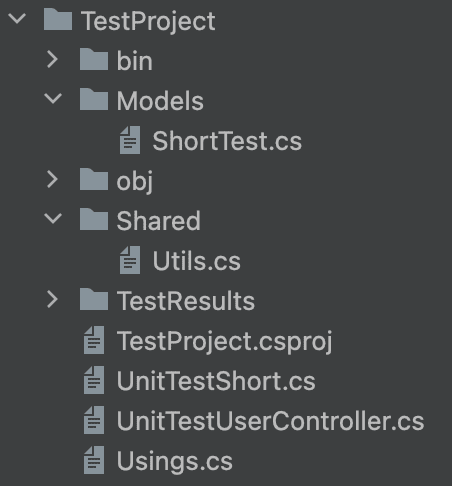
\includegraphics[width=0.5\textwidth]{testproject_structure}
\caption{Структура тестового проекта}
\label{testproject_structure:image}
\end{figure}

Содержимое файла ShortTest.cs представлено на рисунке \ref{st:image}.

\begin{figure}[!ht]
\lstset{style=sharpc}
\begin{lstlisting}
namespace TestProject.Models
{
    [TestClass]
    public class ShortTest
    {
        public long Id { get; set; }
        public string? Name { get; set; }
        public string? Description { get; set; } = null;
    }
}
\end{lstlisting}
\caption{Содержимое файла ShortTest.cs}
\label{st:image}
\end{figure}

Содержимое файла Utils.cs представлено на рисунке \ref{ut:image}.

\begin{figure}[!ht]
\lstset{style=sharpc}
\begin{lstlisting}
namespace TestProject.Shared
{
    public class Utils
    {
        public static void TestString(string v1, string v2)
        {
            if (v1 == null || v2 == null)
            {
                Assert.Fail();
            }

            Assert.AreEqual(v1, v2);
        }

        public static int GenerateUniqueId()
        {
            Random random = new Random();
            return random.Next(1, 101);
        }
    }
}
\end{lstlisting}
\caption{Содержимое файла Utils.cs}
\label{ut:image}
\end{figure}

Содержимое файла Usings.cs представлено на рисунке \ref{usings:image}.

\begin{figure}[!ht]
\lstset{style=sharpc}
\begin{lstlisting}
global using Microsoft.VisualStudio.TestTools.UnitTesting;
global using System.IO;
global using static System.Math;
global using System.Web;
global using Moq;
global using Microsoft.AspNetCore.Mvc;
\end{lstlisting}
\caption{Содержимое файла Usings.cs}
\label{usings:image}
\end{figure}

Модульные тесты для класса Short, который является базовым классом для большинства моделей в приложении, позволяют проверить корректность логики и поведения этого компонента и исключить возникновение проблем в этом классе и его потомков. Тесты охватывают такие аспекты, как валидация имен и описаний, а также уникальность идентификаторов объектов.
Модульные тесты для класса Short представлены на рисунке \ref{unitshort1:image}.

\begin{figure}[ht]
\lstset{style=sharpc}
\begin{lstlisting}
using TestProject.Shared;
using TestProject.Models;

namespace TestProject
{
    [TestClass]
    public class UnitTestShort
    {
        [TestMethod]
        public void Short_Validate_Name()
        {
            var testValue = "Test Name";
            var testObject = new ShortTest() {
                Name = testValue
            };
            Utils.TestString(testObject.Name, testValue);
        }

        [TestMethod]
        public void Short_Validate_Description()
        {
            var testValue = "Test description";
            var testObject = new ShortTest() {
                Description = testValue
            };
            Utils.TestString(testObject.Description, testValue);
        }

        [TestMethod]
        public void Short_Validate_Id()
        {
            var testObject = new ShortTest();
            long randomId = 0;
            while (randomId == 0)
            {
                randomId = Utils.GenerateUniqueId();
            }
            testObject.Id = randomId;
            Assert.AreNotEqual(0, testObject.Id);
            Assert.AreEqual(randomId, testObject.Id);
        }
    }
}  
\end{lstlisting}
\caption{Модульный тест класса Short}
\label{unitshort1:image}
\end{figure}

Для контроллера UserController, который обрабатывает пользовательские запросы, были разработаны тесты, имитирующие взаимодействие с репозиторием данных. Это позволяет тестировать контроллер в изоляции от реальной базы данных, что упрощает процесс разработки и повышает качество кода.
Модульные тесты для UserController представлены в двух частях на рисунках \ref{unitcontr1:image} и \ref{unitcontr2:image}.

\begin{figure}[ht]
\lstset{style=sharpc}
\begin{lstlisting}
global using new_back.Controllers;
global using new_back.Infrastructure;
global using new_back.Models;

namespace TestProject
{
    [TestClass]
    public class UserControllerTests
    {
        private Mock<IUserRepository> _mockRepository;
        private UserController _controller;

        [TestInitialize]
        public void SetUp()
        {
            _mockRepository = new Mock<IUserRepository>();
            _controller = new UserController(_mockRepository.Object);
        }

        [TestMethod]
        public void GetById_UserExists_ReturnsUserView()
        {
            long userId = 1;
            var mockUser = new User { Id = userId, Email = "test@example.com" };
            _mockRepository.Setup(repo => repo.GetById(userId)).Returns(mockUser);

            var result = _controller.GetById(userId);

            Assert.IsNotNull(result);
            Assert.IsInstanceOfType(result.Result, typeof(OkObjectResult));

            var okResult = result.Result as OkObjectResult;
            Assert.IsNotNull(okResult);

            var userViewResult = okResult.Value as UserView;
            Assert.IsNotNull(userViewResult);
            Assert.AreEqual(userId, userViewResult.Id);
            Assert.AreEqual("test@example.com", userViewResult.Email);
        }
\end{lstlisting}
\caption{Модульный тест класса UserController часть 1}
\label{unitcontr1:image}
\end{figure}


\begin{figure}[ht]
\lstset{style=sharpc}
\begin{lstlisting}
    [TestMethod]
    public void GetById_UserDoesNotExist_ReturnsNotFound()
    {
        _mockRepository.Setup(repo => repo.GetById(It.IsAny<long>())).Returns((User)null);

        var result = _controller.GetById(1);

        Assert.IsInstanceOfType(result.Result, typeof(NotFoundResult));
    }
  }
}
\end{lstlisting}
\caption{Модульный тест класса UserController часть 2}
\label{unitcontr2:image}
\end{figure}

Разработка тестового проекта является ключевым компонентом в цикле обеспечения качества программного продукта. Она демонстрирует эффективность тестирования и его способность гарантировать надежность функционирования системы. На рисунке \ref{testresult:image} представлены результаты выполнения модульных тестов, подтверждающие успешную проверку всех компонентов системы, что свидетельствует об отсутствии критических ошибок и готовности продукта к дальнейшим этапам разработки и внедрения.

 % при необходимости можно переносить рисунок на новую страницу
\begin{figure}[H] % H - рисунок обязательно здесь, или переносится, оставляя пустоту
\centering
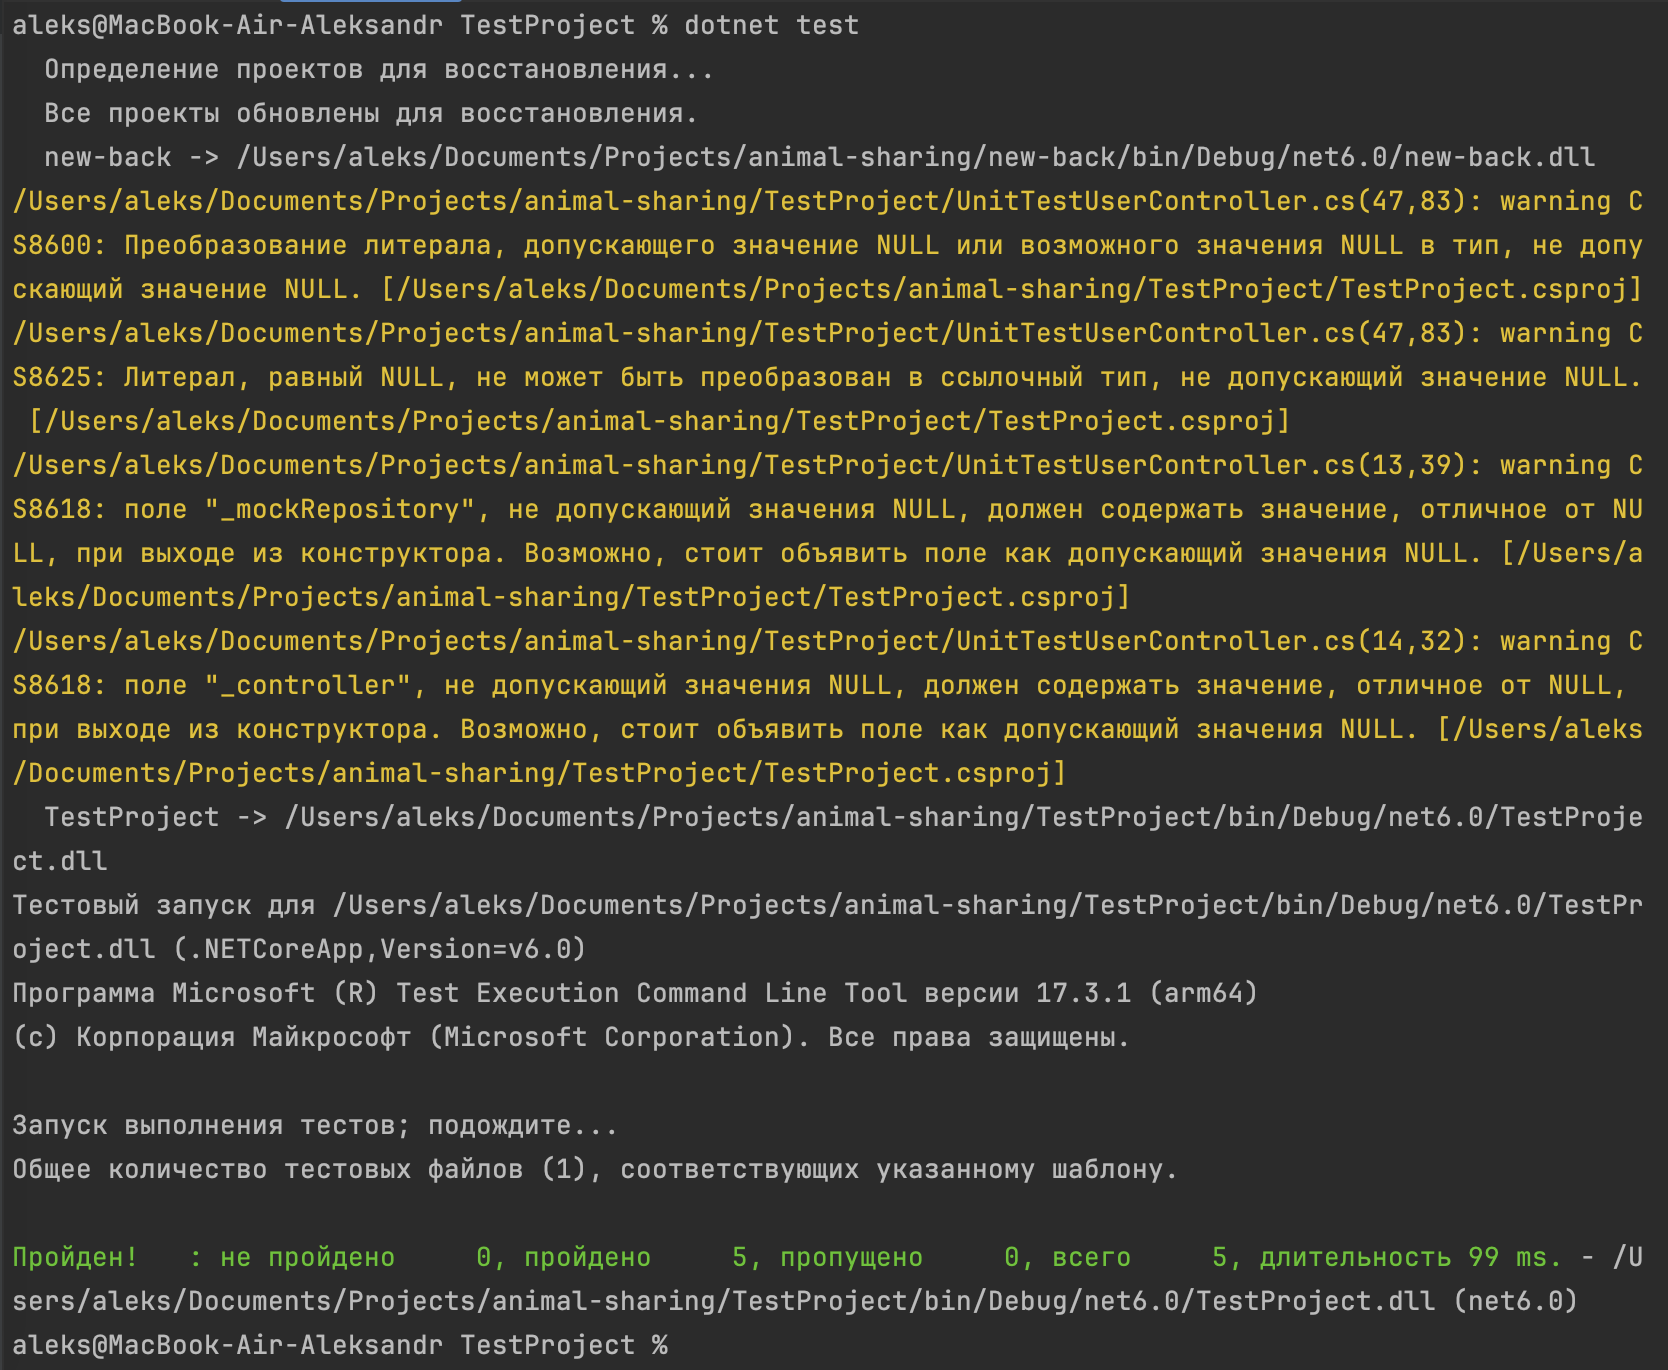
\includegraphics[width=0.8\textwidth]{testresult}
\caption{Результаты выполнения модульных тестов}
\label{testresult:image}
\end{figure}

\subsection{Системное тестирование разработанного веб-приложения}

Каждая страница веб-приложения включает в себя такие элементы интерфейса как шапка сайта, боковое меню и основное содержимое страницы.

Шапка сайта состоит из:
\begin{itemize}
    \item кнопка для раскрытия или закрытия бокового меню в зависимости от его текущего состояния;
    \item логотип;
    \item кнопки для перехода на страницу входа в систему и регистрации или имя и фамилию пользователя если он авторизован в системе и кнопку выхода пользователя из системы.
\end{itemize}

Боковое меню включает в себя ссылки на различные страницы сайта.
Основное содержимое страницы меняется в зависимости от выбранного раздела сайта и включает в себя заголовок страницы и ее содержимое. 

Главная страница включает в себя список карточек продуктов (товаров и услуг), шапку сайта и боковое меню. Пользователь может просматривать карточки продуктов (товаров и услуг), а также раскрывать при нажатии на кнопку <<Подробнее>> раскрывать блок с детальной информацией о товаре или услуге.
На рисунке \ref{test-front1:image} представлена главная страница веб-приложения для неавторизованного пользователя с открытым боковым меню. Первая карточка с услугой <<Кошки в аренду>> раскрыта для просмотра детальной информации.

\begin{figure}[H] % H - рисунок обязательно здесь, или переносится, оставляя пустоту
\center{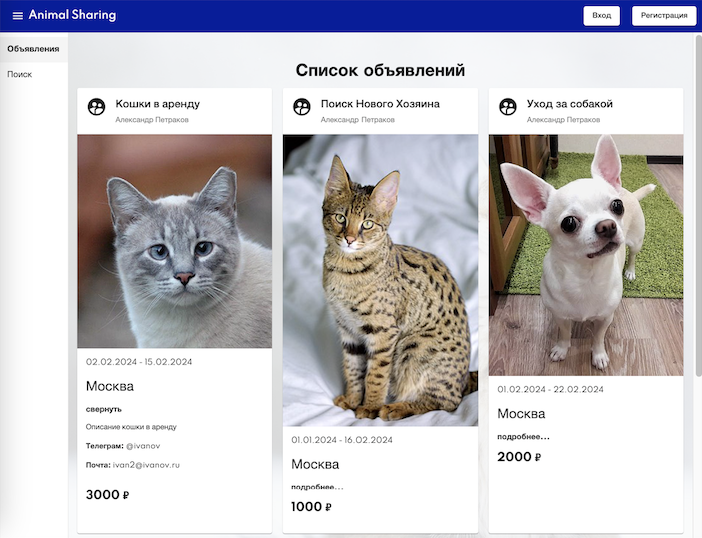
\includegraphics[width=1\linewidth]{test-front1}}
\caption{Главная страница веб-приложения}
\label{test-front1:image}
\end{figure}

На рисунке \ref{test-front2:image} представлена страница регистрации пользователя-поставщика услуг. На рисунке \ref{test-front2:image} также изображено боковым меню в закрытом состоянии.

 % при необходимости можно переносить рисунок на новую страницу
\begin{figure}[H] % H - рисунок обязательно здесь, или переносится, оставляя пустоту
\center{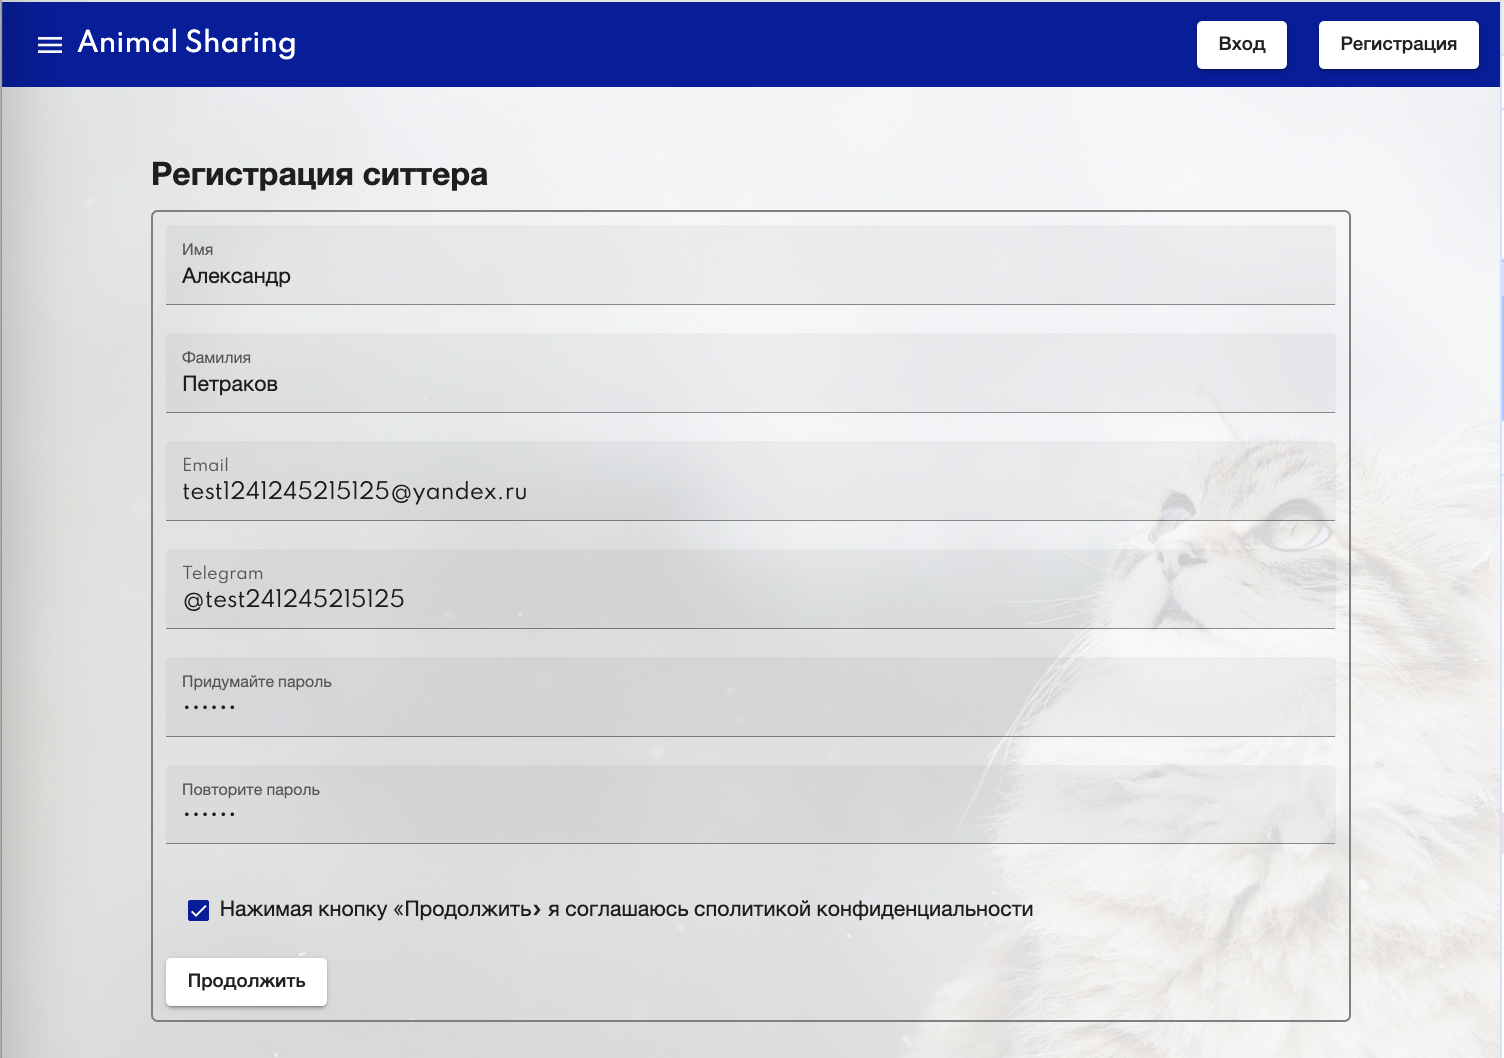
\includegraphics[width=1\linewidth]{test-front2}}
\caption{Страница регистрации пользователя-поставщика услуг}
\label{test-front2:image}
\end{figure}

После регистрации пользователь автоматически авторизуется в системе и перенаправляется на главную страницу приложения где он может просматривать карточки продуктов (товаров и услуг), а также создавать свои карточки. На рисунке \ref{test-front3:image} представлена страница создания карточки. На рисунке \ref{test-front3:image} также изображено состояние шапки сайта для авторизованного пользователя.

 % при необходимости можно переносить рисунок на новую страницу
\begin{figure}[H] % H - рисунок обязательно здесь, или переносится, оставляя пустоту
\center{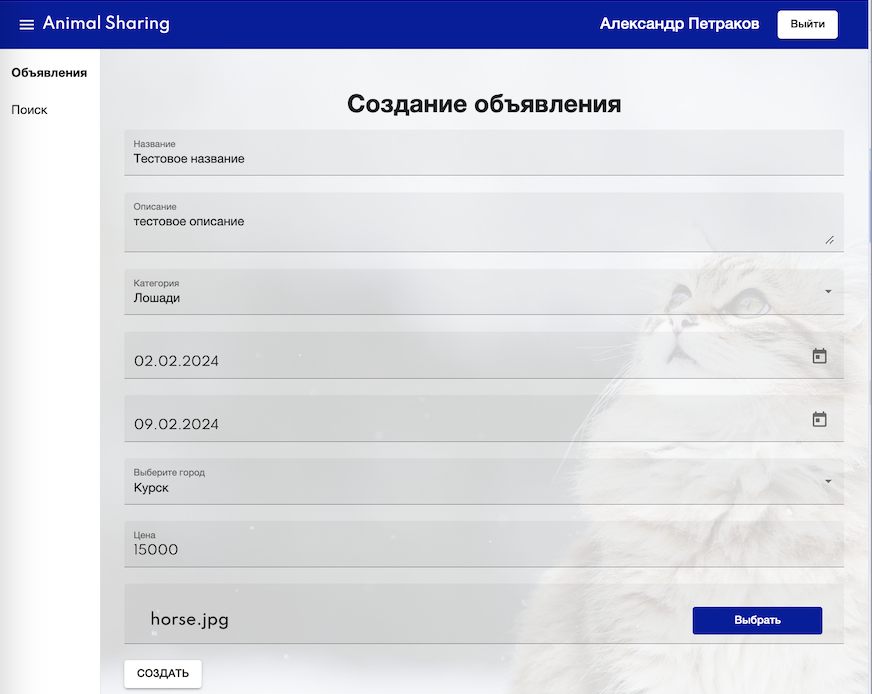
\includegraphics[width=1\linewidth]{test-front3}}
\caption{Страница регистрации создания карточки}
\label{test-front3:image}
\end{figure}

Созданная карточка отображается на главной странице веб-приложения. На рисунке \ref{test-front4:image} представлена главная страница веб-приложения для авторизованного пользователя с открытым боковым меню. Новая карточка с названием <<Тестовое название>> содержит кнопку для редактирования при нажатии на которую пользователь перенаправляется на страницу редактирования этой карточки. Новая карточка также содержит кнопку удаления. На рисунке \ref{test-front4:image} изображена обновленная главная страница веб-приложения.

 % при необходимости можно переносить рисунок на новую страницу
\begin{figure}[H] % H - рисунок обязательно здесь, или переносится, оставляя пустоту
\center{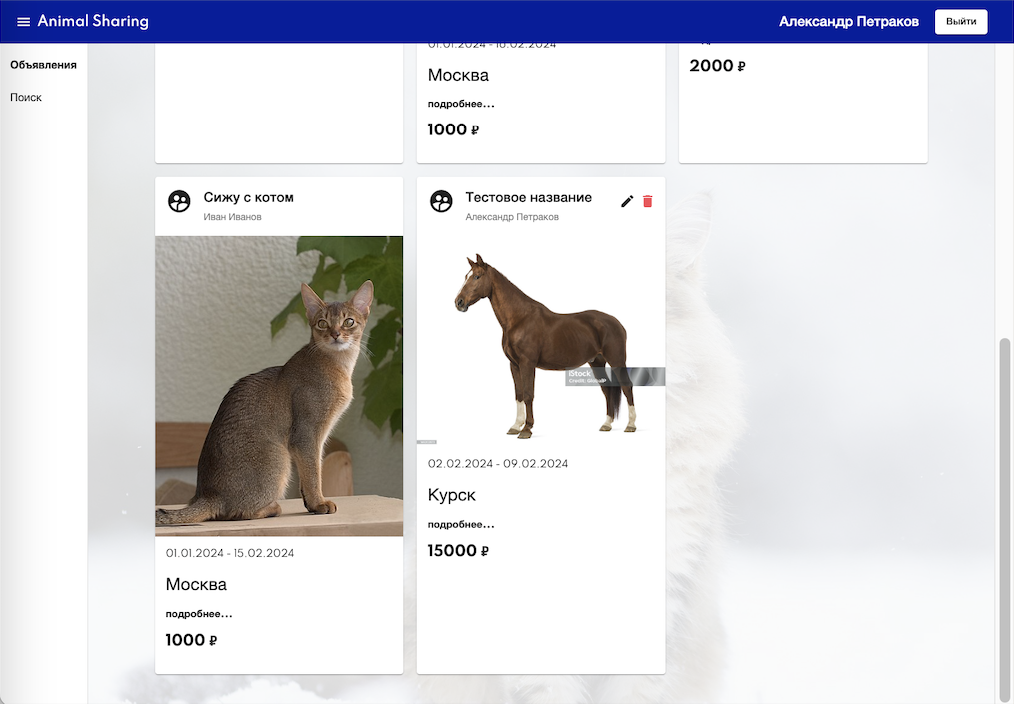
\includegraphics[width=1\linewidth]{test-front4}}
\caption{Обновленная главная страница веб-приложения}
\label{test-front4:image}
\end{figure}

На рисунке \ref{test-front5:image} изображена страница редактирования карточки с новым выбранным изображением товара в поле <<Изображение>>. На рисунке \ref{test-front6:image} изображена страница редактирования карточки после нажатия на кнопку <<Сохранить>>.

 % при необходимости можно переносить рисунок на новую страницу
\begin{figure}[H] % H - рисунок обязательно здесь, или переносится, оставляя пустоту
\center{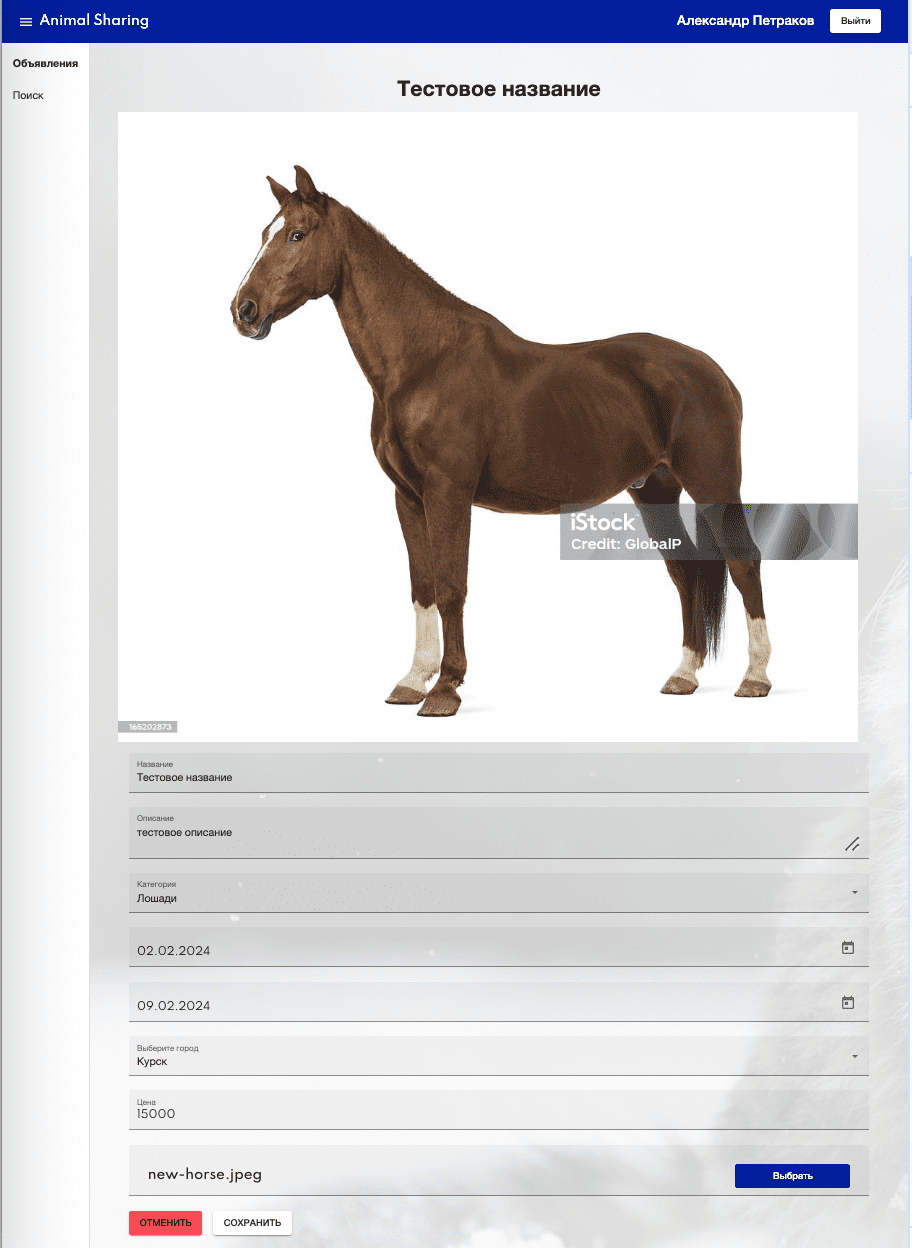
\includegraphics[width=1\linewidth]{test-front5}}
\caption{Страница редактирования карточки}
\label{test-front5:image}
\end{figure}

 % при необходимости можно переносить рисунок на новую страницу
\begin{figure}[H] % H - рисунок обязательно здесь, или переносится, оставляя пустоту
\center{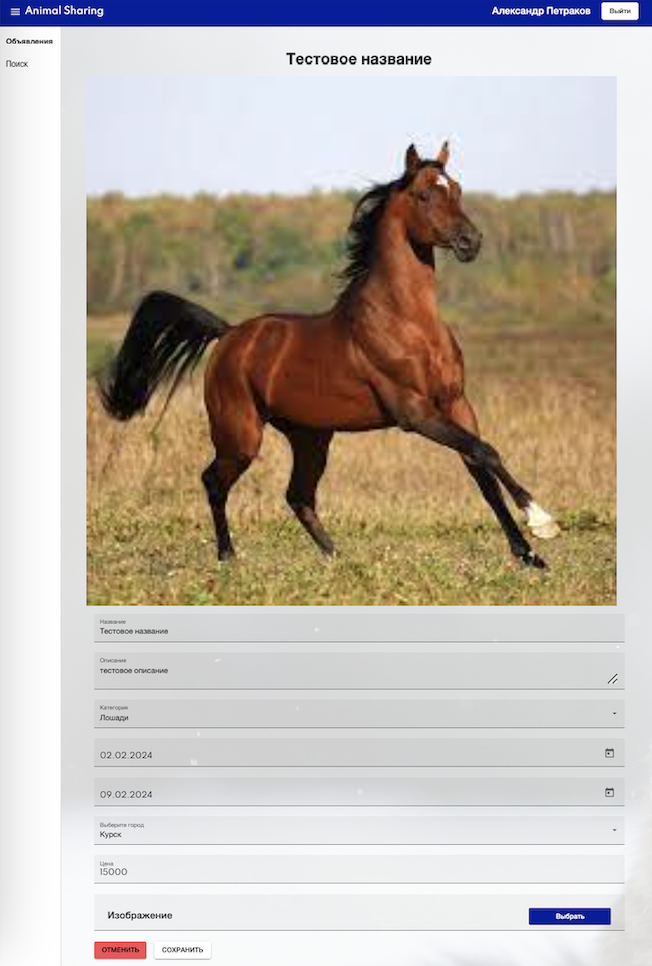
\includegraphics[width=1\linewidth]{test-front6}}
\caption{Обновленная страница редактирования карточки}
\label{test-front6:image}
\end{figure}

На рисунке \ref{test-front7:image} изображена страница поиска с предустановлеными фильтрами. На рисунке \ref{test-front8:image} изображена страница с результатами поиска по заданным на странице поиска фильтрам.

\begin{figure}[H] % H - рисунок обязательно здесь, или переносится, оставляя пустоту
\center{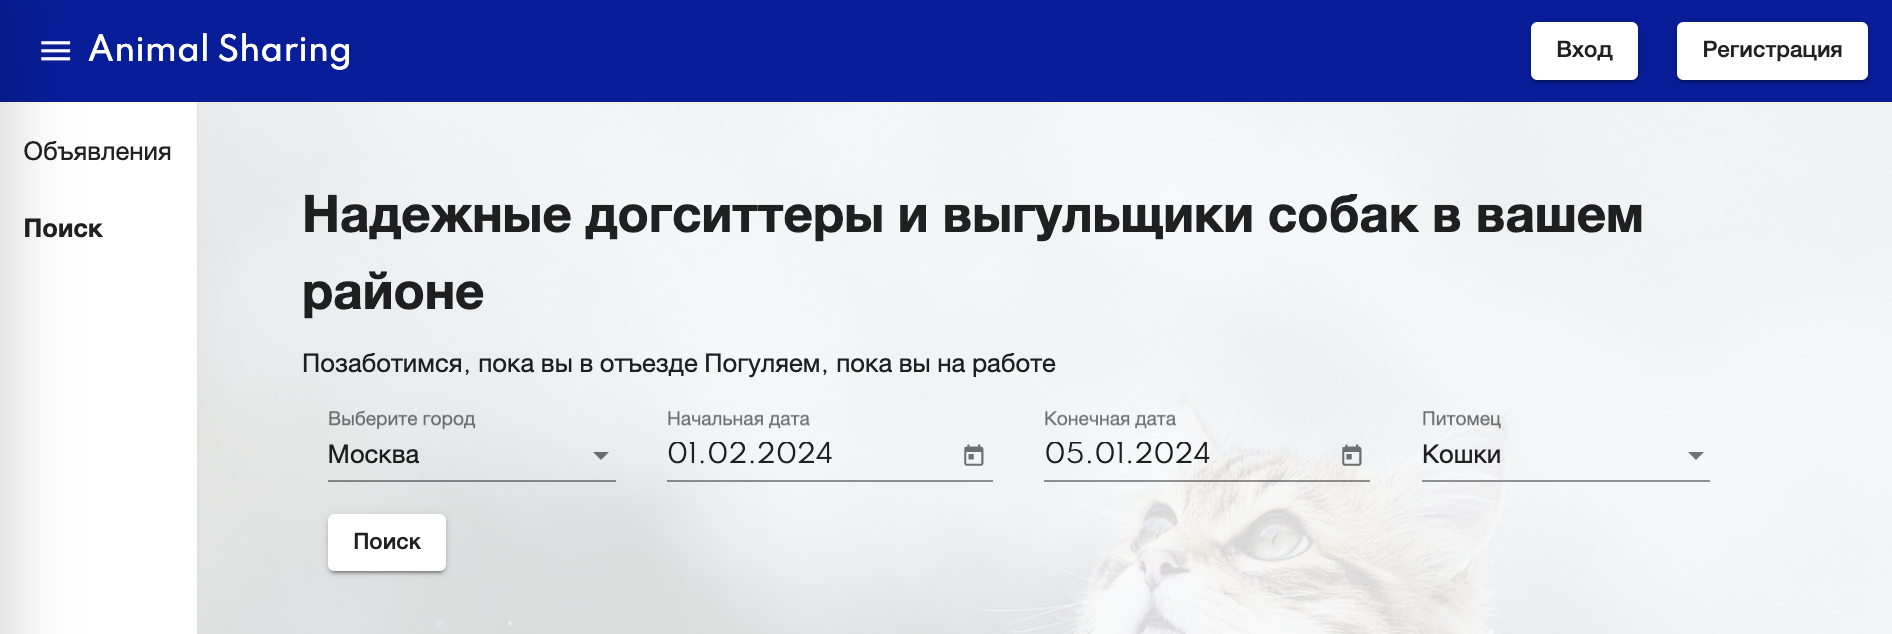
\includegraphics[width=1\linewidth]{interface-search}}
\caption{Страница поиска}
\label{test-front7:image}
\end{figure}

\begin{figure}[H] % H - рисунок обязательно здесь, или переносится, оставляя пустоту
\center{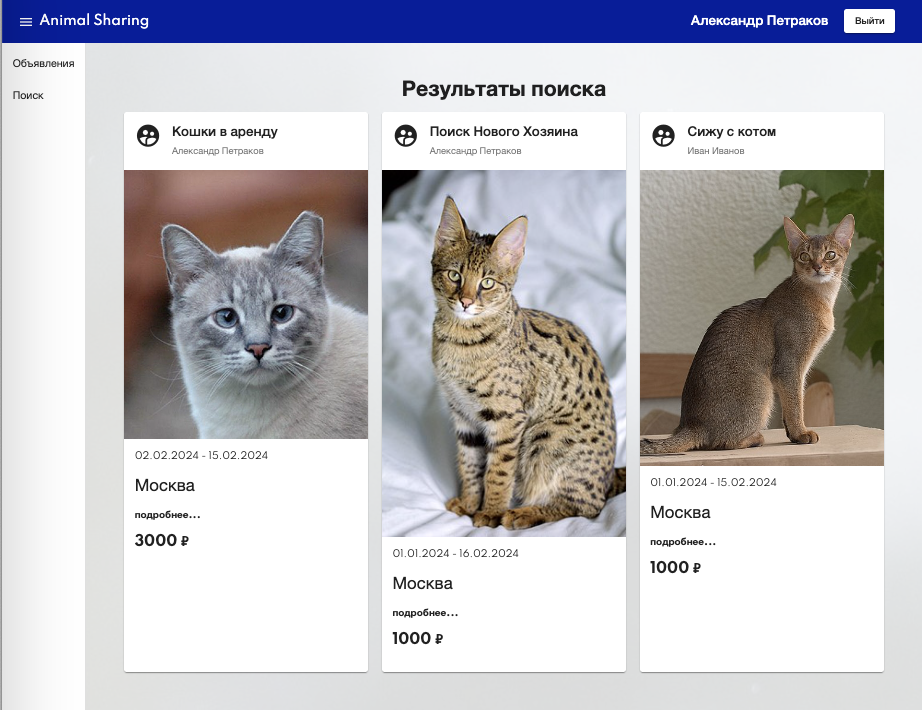
\includegraphics[width=1\linewidth]{test-front8}}
\caption{Страница с результатами поиска}
\label{test-front8:image}
\end{figure}

Убедимся в корректности работы поиска. На рисунке \ref{test-front-20:image} изображена страница поиска с измененными фильтрами, а на рисунке \ref{test-front-21:image} изображена страница с результатами поиска после выбора новых фильтров и нажатия кнопки <<Поиск>>.

\begin{figure}[H] % H - рисунок обязательно здесь, или переносится, оставляя пустоту
\center{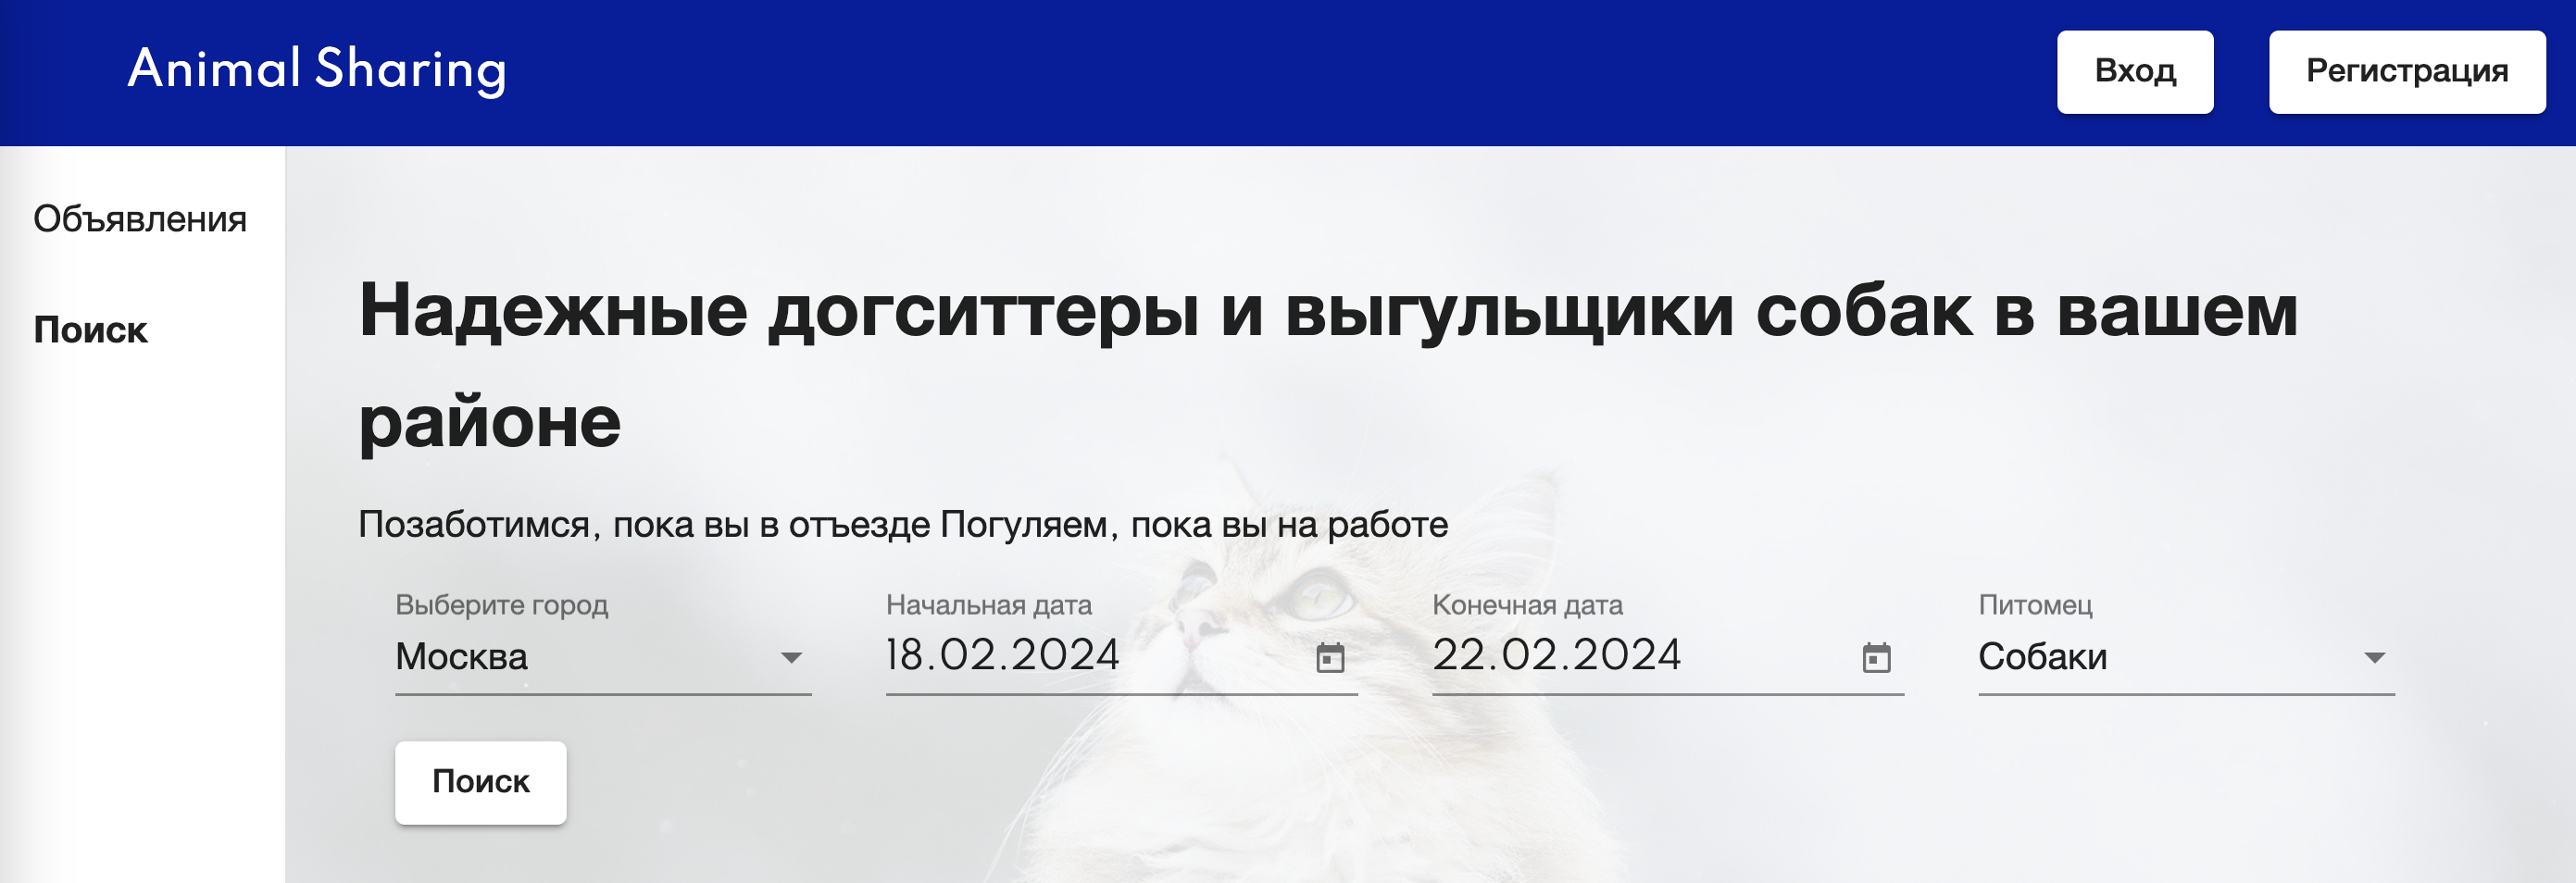
\includegraphics[width=1\linewidth]{test-front-20}}
\caption{Страница поиска с измененными фильтрами}
\label{test-front-20:image}
\end{figure}

\begin{figure}[H] % H - рисунок обязательно здесь, или переносится, оставляя пустоту
\center{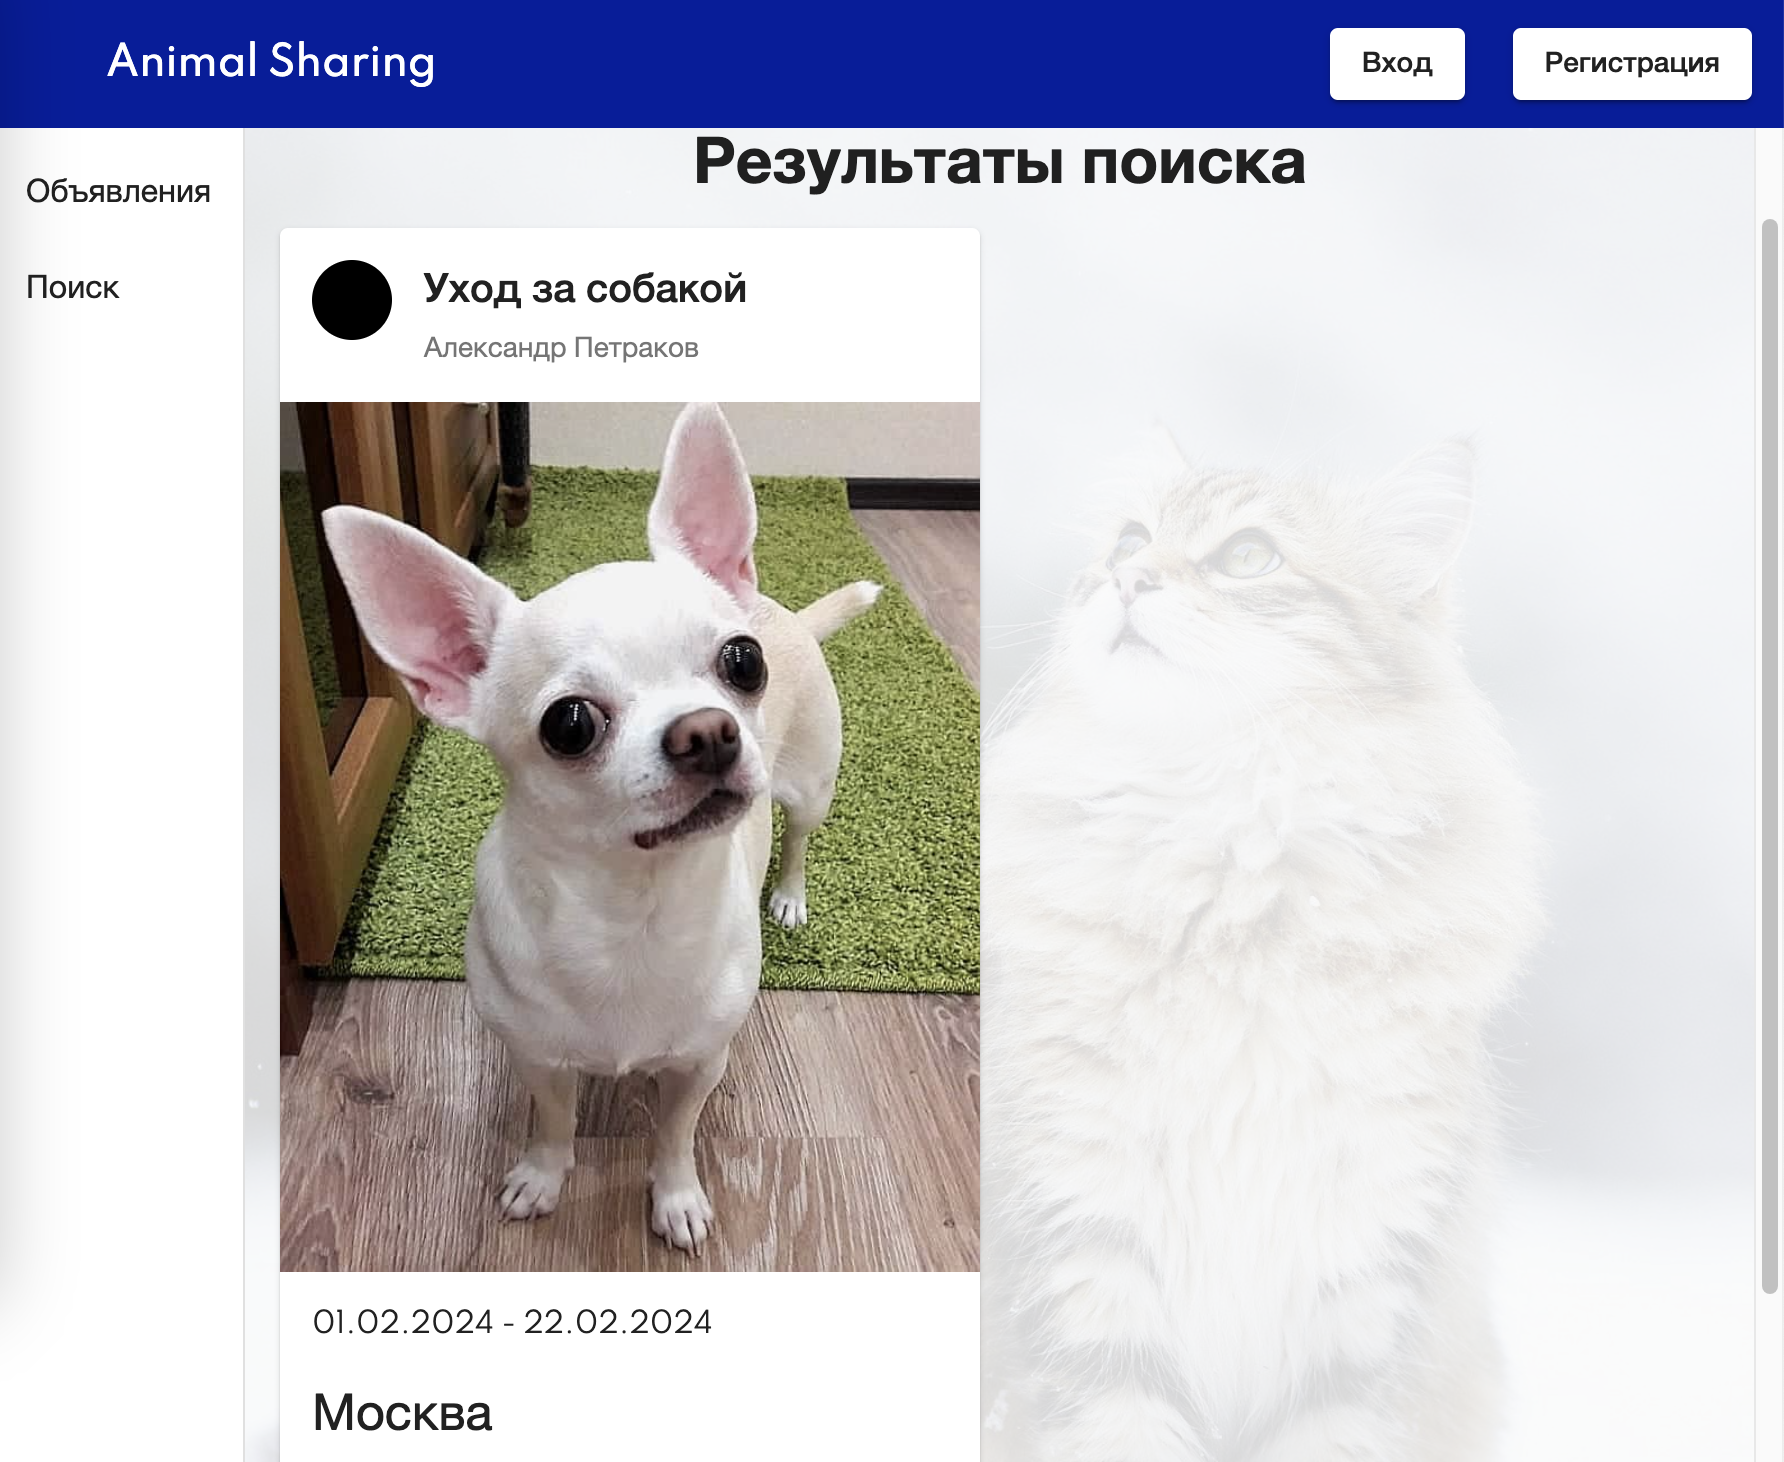
\includegraphics[width=1\linewidth]{test-front-21}}
\caption{Страница с результатами поиска для новых фильтров}
\label{test-front-21:image}
\end{figure}

Вернемся на главную страницу веб-приложения. На рисунке \ref{test-front-1:image} в виде иконок представлены следующие элементы управления карточкой:

\begin{itemize}
  \item иконка с карандашом при нажатии на которую пользователь переходит на страницу редактирования карточки, что уже было протестировано и представлено на рисунке \ref{test-front5:image}.
  \item иконка корзины -\- удаляет созданную ранее карточку.
\end{itemize}

\begin{figure}[H] % H - рисунок обязательно здесь, или переносится, оставляя пустоту
  \center{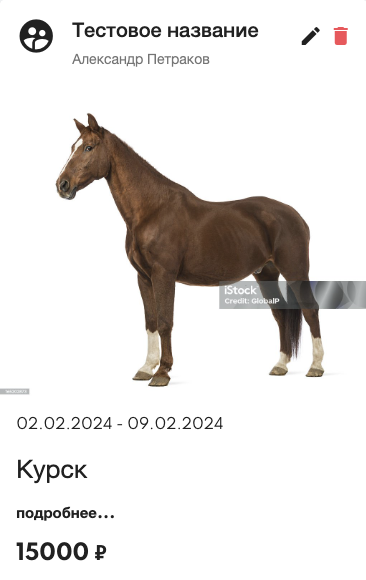
\includegraphics[width=0.75\linewidth]{test-front-1}}
  \caption{Элементы управления карточкой}
  \label{test-front-1:image}
\end{figure}

На рисунке \ref{test-front15:image} изображена главная страница веб-приложения после удаления карточки.

\begin{figure}[H] % H - рисунок обязательно здесь, или переносится, оставляя пустоту
  \center{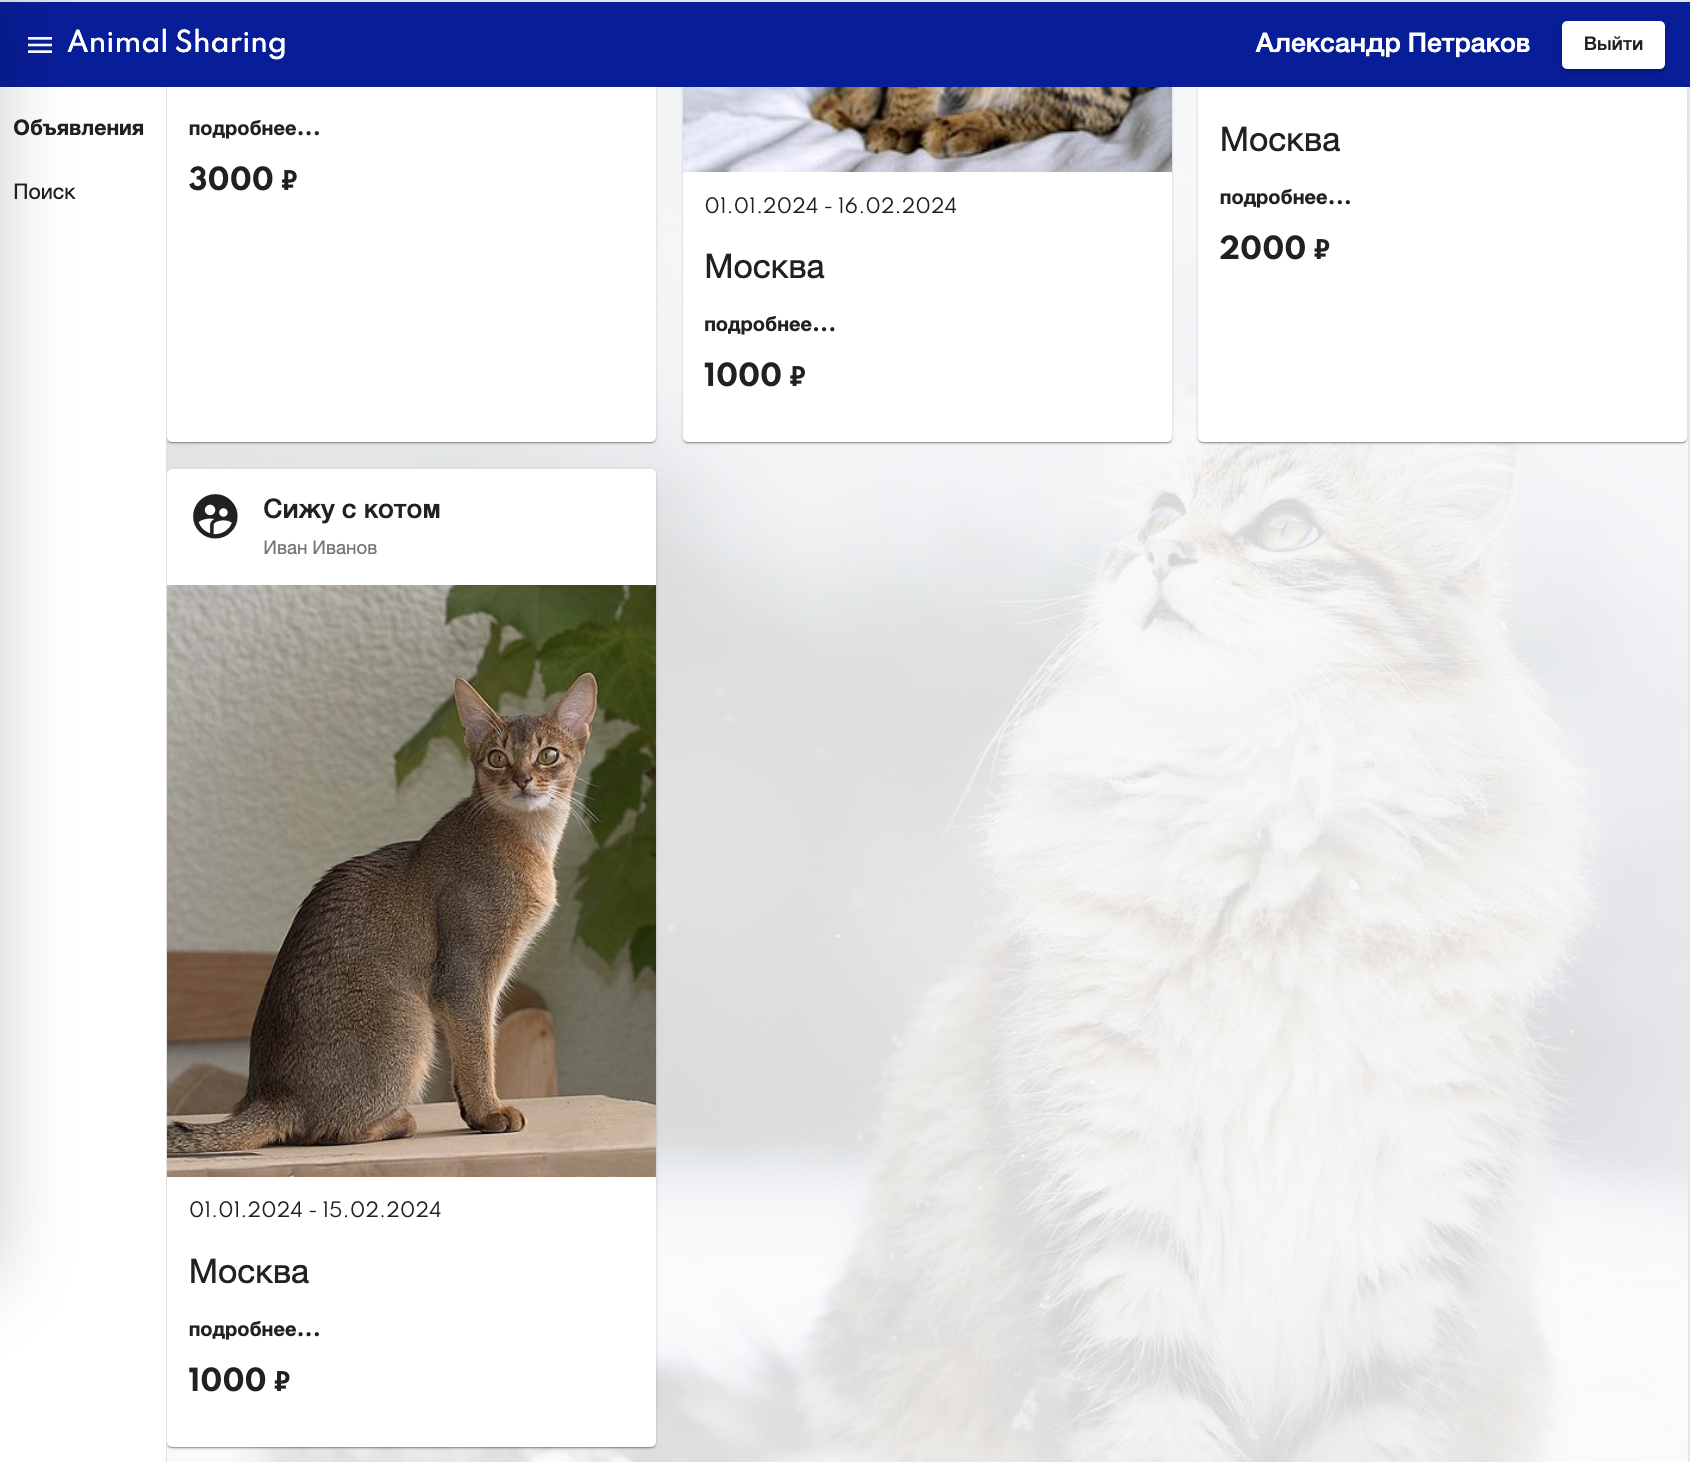
\includegraphics[width=1\linewidth]{test-front-15}}
  \caption{Обновленная главная страница после удаления карточки}
  \label{test-front15:image}
\end{figure}
  